\section{The four- and five-piece estimates}\label{app:terminal-estimates}

This appendix proves \cref{thm:four-density,thm:five-density}. Both reduce to functions of one
variable, and both rest on the same elementary bound for the logarithm.

\subsection{A logarithm bound}\label{app:log-bound}

\begin{lemma}\label{lem:log-sinh}
For $0<x\le1$, $\ \dfrac{x-x^{-1}}{2}\le\log x$.
\end{lemma}

\begin{proof}
With $y=-\log x\ge0$ the inequality reads $y\le\sinh y$.
\end{proof}

The two sides agree to second order at $x=1$: both are $(x-1)-\tfrac12(x-1)^2+O((x-1)^3)$. This
is what makes the bound useful near the octagon, where the parameters below approach the points
at which the estimates are sharp.

\subsection{The four-piece density}\label{app:four-density}

Recall $\delta(a,b)$ from \eqref{eq:four-density}, on the open quarter circle $a,b>0$,
$a^2+b^2=1$, with $s=a+b$.

\begin{lemma}[A monotone weight]\label{lem:four-weight}
For $c\ge2$ the function $w_c(x)=(2x+c)\log x/(1-x)$ is nondecreasing on $(0,1)$. Consequently,
for $0<b\le a<1$,
\[
 (2b+c)(1-a)\log b\ \le\ (2a+c)(1-b)\log a.
\]
\end{lemma}

\begin{proof}
The derivative is $w_c'(x)=\bigl((2+c)\log x+(2x+c)(1-x)/x\bigr)/(1-x)^2$. By
\cref{lem:log-sinh} and $2+c>0$, the numerator is at least
\[
 (2+c)\frac{x-x^{-1}}{2}+\frac{(2x+c)(1-x)}{x}=\frac{(c-2)(1-x)^2}{2x}\ \ge\ 0.
\]
The second statement is $w_c(b)\le w_c(a)$ multiplied by $(1-a)(1-b)>0$.
\end{proof}

\begin{proof}[Proof of \cref{thm:four-density}]
Since $\delta(a,b)=\delta(b,a)$, we may assume $b\le a$, that is $b\in(0,1/\sqrt2\,]$ and
$a=\sqrt{1-b^2}$. Put $\psi(b)=\delta(\sqrt{1-b^2},b)$. For $0<b<1/\sqrt2$, differentiating
\eqref{eq:four-density} with $a'=-b/a$ and simplifying on the circle gives, with $c=2+2ab$,
\begin{equation}\label{eq:four-derivative}
 \psi'(b)=\frac{2\Bigl((s+1)\bigl(w_c(b)-w_c(a)\bigr)-s(s-1)(a-b)\Bigr)}{a\,(s+1)\,(s+3)^2}.
\end{equation}
Here $c\ge2$ and $b<a$, so $w_c(b)\le w_c(a)$ by \cref{lem:four-weight}, while $s>1$ and $a>b$
make the last term negative. Hence $\psi'<0$ on $(0,1/\sqrt2)$, and $\psi$, which is continuous
at $1/\sqrt2$, is strictly decreasing on $(0,1/\sqrt2\,]$. For $b<1/\sqrt2$ this gives
$\delta(a,b)=\psi(b)>\psi(1/\sqrt2)=\doct$, the value computed after \cref{thm:four-density}.
So $\delta(a,b)\ge\doct$ with equality only at $a=b$.
\end{proof}

The computation behind \eqref{eq:four-derivative} is mechanical. Write $\delta=\mathcal D/\mathcal N$
with $\mathcal D$ the numerator of \eqref{eq:four-density} and $\mathcal N=(s-1)(s+3)$, and let a
prime denote $\dd/\dd b$ along the circle, so that $a'=-b/a$ and $s'=(a-b)/a$. By the quotient
rule, $\psi'(b)=\kappa/(a^2b\,\mathcal N^2)$ with $\kappa=a^2b\,(\mathcal D'\mathcal N-\mathcal D\,\mathcal N')$,
a polynomial in $a$, $b$, $\log a$ and $\log b$, and modulo $a^2+b^2-1$ it satisfies
\[
 \kappa\,(1-a)(1-b)(s+1)
 =2ab(s-1)^2\Bigl((s+1)\,\Delta-(a-b)\,s\,(s-1)(1-a)(1-b)\Bigr),
\]
where $\Delta=(2b+c)(1-a)\log b-(2a+c)(1-b)\log a$ is the quantity of \cref{lem:four-weight}.
Since $\Delta=(1-a)(1-b)\bigl(w_c(b)-w_c(a)\bigr)$ and $\mathcal N^2=(s-1)^2(s+3)^2$, this is
\eqref{eq:four-derivative}.

\subsection{The five-piece density}\label{app:five-density}

Recall $F$, $d=(1-u)(1-v)$ and $\delta(u,v)$ from \eqref{eq:five-density}, and put
$t_*=\sqrt2-1$, $d_*=(2-\sqrt2)^2$ and $\mathcal K=(3+2\sqrt2)\log2$. Since
$(3+2\sqrt2)(2-\sqrt2)^2=2$, we have $\mathcal K d_*=2\log2$.

The function $F$ is not concave (\texttt{FIVE\_ARC\_PROGRESS}, \S7), so its maximum cannot be
read off from a second derivative. It becomes tractable after a change of variables that splits
it into two values of one concave function at two points of the unit circle.

\begin{lemma}[A concave function]\label{lem:five-h}
Let $h(t)=-2t\log t/(1-t)-\log(1+t)$ for $0<t<1$. Then $x\mapsto h(\sqrt x)$ is concave on
$(0,1)$. Consequently $h(\alpha)+h(\beta)\le2h(1/\sqrt2)$ whenever $\alpha,\beta>0$ and
$\alpha^2+\beta^2=1$.
\end{lemma}

\begin{proof}
Put $E(t)=t-1-\log t\ge0$. Then $h'(t)=2E/(1-t)^2-1/(1+t)$, and the derivative of $h(\sqrt x)$
is $k(\sqrt x)/2$ with $k(t)=h'(t)/t$, so it suffices that $k$ is nonincreasing. Now
$k'(t)=(th''(t)-h'(t))/t^2$ and
\[
 th''-h'=-\frac{2}{1-t}+\frac{2(3t-1)E}{(1-t)^3}+\frac{1+2t}{(1+t)^2}
 =\frac{\mathcal M(t)}{(1-t)^3(1+t)^2},
\]
\[
 \mathcal M(t)=-2(1-t)^2(1+t)^2+2(3t-1)E(1+t)^2+(1+2t)(1-t)^3 .
\]
If $t\le1/3$, the middle term of $\mathcal M$ is at most $0$, and the other two add up to
$-(1-t)^2(1+3t+4t^2)<0$. If $t>1/3$, \cref{lem:log-sinh} gives
$E\le t-1-\tfrac12(t-t^{-1})=(1-t)^2/(2t)$, so $2tE\le(1-t)^2$ and
\begin{align*}
 t\,\mathcal M(t)&\le-2t(1-t)^2(1+t)^2+(3t-1)(1+t)^2(1-t)^2+t(1+2t)(1-t)^3\\
 &=(1-t)^3(t^2-t-1)<0.
\end{align*}
For the second statement apply concavity at $x=\alpha^2$ and $x=\beta^2$ with weights $\tfrac12$:
$\tfrac12h(\alpha)+\tfrac12h(\beta)\le h\bigl(\sqrt{(\alpha^2+\beta^2)/2}\bigr)=h(1/\sqrt2)$.
\end{proof}

\begin{lemma}[The envelope]\label{lem:five-envelope}
For $0<t<1$,
\[
 F(t)+2\log(1-t)\ \le\ \mathcal K+2\log(2-\sqrt2)=\mathcal K+\log d_*.
\]
\end{lemma}

The bound is attained at $t=t_*$: there $(1+t^2)/(2t)=(1+t^2)/(1-t^2)=\sqrt2$,
$2t/(1-t^2)=1$ and $(1+t)/(1-t)=1/t=\sqrt2+1$, so $F(t_*)=(3+2\sqrt2)\log2=\mathcal K$, and
$1-t_*=2-\sqrt2$.

\begin{proof}
With $\alpha=2t/(1+t^2)$ and $\beta=(1-t^2)/(1+t^2)$, so that $\alpha^2+\beta^2=1$, expanding
the logarithms of the products $1-\alpha=(1-t)^2/(1+t^2)$, $1+\alpha=(1+t)^2/(1+t^2)$,
$1-\beta=2t^2/(1+t^2)$ and $1+\beta=2/(1+t^2)$ gives the identity
\[
 F(t)+2\log(1-t)=\log2+h(\alpha)+h(\beta).
\]
By \cref{lem:five-h} this is at most $\log2+2h(1/\sqrt2)$. Since $\log(1/\sqrt2)=-\tfrac12\log2$
and $1+1/\sqrt2=(2+\sqrt2)/2=1/(2-\sqrt2)$,
\[
 h(1/\sqrt2)=\frac{\sqrt2\cdot\tfrac12\log2}{1-1/\sqrt2}-\log\frac{1}{2-\sqrt2}
 =(1+\sqrt2)\log2+\log(2-\sqrt2),
\]
so $\log2+2h(1/\sqrt2)=(3+2\sqrt2)\log2+2\log(2-\sqrt2)$.
\end{proof}

\begin{lemma}\label{lem:five-d}
If $u,v\in(0,1)$ and $u+v+uv>1$, then $d=(1-u)(1-v)<d_*$.
\end{lemma}

\begin{proof}
Put $x=1-u$, $y=1-v$ and $\omega=\sqrt{xy}$. The hypothesis is $(2-x)(2-y)>2$, that is,
$2-2(x+y)+xy>0$. Since $x+y\ge2\omega$, also $\omega^2-4\omega+2>0$, so $\omega<2-\sqrt2$ or
$\omega>2+\sqrt2$; the second is impossible because $\omega<1$. Hence $d=\omega^2<d_*$.
\end{proof}

\begin{proof}[Proof of \cref{thm:five-density}]
Adding \cref{lem:five-envelope} at $t=u$ and $t=v$, and using
$\log d=\log(1-u)+\log(1-v)$,
\[
 F(u)+F(v)\le2\mathcal K+2\log d_*-2\log d .
\]
Multiplying by $d/2>0$,
\[
 (4-d)\,\delta(u,v)=2d+4-\tfrac d2\bigl(F(u)+F(v)\bigr)\ \ge\ 2d+4-\mathcal Kd-d\log d_*+d\log d .
\]
The tangent line of $d\mapsto d\log d$ at $d_*$ gives $d\log d\ge d\log d_*+d-d_*$ (this is
$\log(d/d_*)\ge1-d_*/d$), so
\[
 (4-d)\,\delta(u,v)\ \ge\ 4-d_*+(3-\mathcal K)\,d .
\]
At $d=d_*$ the right side equals $\doct(4-d_*)$: indeed $2d_*+4-\mathcal Kd_*=16-8\sqrt2-2\log2$
and $4-d_*=2(2\sqrt2-1)$. Subtracting $\doct(4-d)=\doct(4-d_*)+\doct(d_*-d)$,
\[
 (4-d)\bigl(\delta(u,v)-\doct\bigr)\ \ge\ (\mathcal K-3-\doct)(d_*-d).
\]
Both factors on the right are positive: $d<d_*$ by \cref{lem:five-d}, and
$\mathcal K=4.0400\ldots>3+\doct=3.9024\ldots$; indeed $\sqrt2>1.4142$ and $\log2>0.6931$ give
$\mathcal K>4.039$ and $\doct<0.9025$. Since $4-d>0$, $\delta(u,v)>\doct$.
\end{proof}

\begin{remark}
Another way to finish \cite{Notes}: with $M=\mathcal K+\log d_*$, the bound obtained from
\cref{lem:five-envelope} is $\delta(u,v)\ge B(d)=\bigl(2(d+2)-d(M-\log d)\bigr)/(4-d)$, and
\[
 B'(d)=\frac{4(4-M+\log d)-d}{(4-d)^2}<0\qquad(0<d\le d_*),
\]
because $4-M+\log d\le4-\mathcal K<0$ there. So $B$ decreases on $(0,d_*]$ to
$B(d_*)=\doct$. The inequality $\mathcal K>4$ also follows from the rational bounds $\sqrt2>7/5$
and $\log2>56/81$.
\end{remark}

\begin{figure}[htbp]
 \centering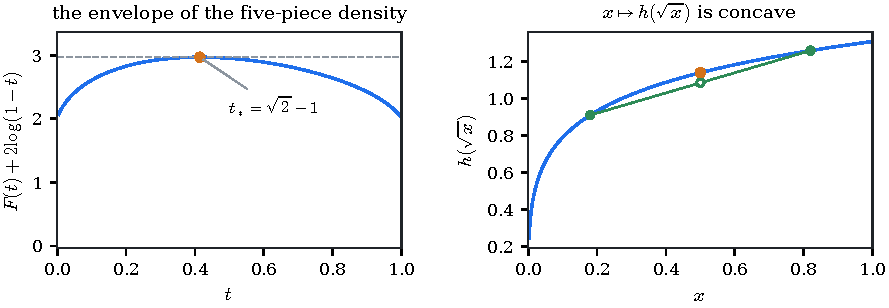
\includegraphics[width=\textwidth]{figures/fig-terminal-envelope.pdf}
 \caption{Left: $F(t)+2\log(1-t)$ on $(0,1)$; its maximum
 $(3+2\sqrt2)\log2+2\log(2-\sqrt2)=2.970\ldots$ is attained only at $t_*=\sqrt2-1$
 (\cref{lem:five-envelope}). Right: the concave function $x\mapsto h(\sqrt x)$ of
 \cref{lem:five-h}; a chord (green) lies below the graph, and the midpoint of the chord between
 $\alpha^2$ and $\beta^2=1-\alpha^2$ lies below the value at $x=1/2$ (orange). Computed; the
 script checks the identity $F(t)+2\log(1-t)=\log2+h(\alpha)+h(\beta)$ and the concavity on a
 grid.}
 \label{fig:terminal-envelope}
\end{figure}
